\documentclass{article}
\usepackage[dblblindworkshop]{neurips_2026}
\workshoptitle{Foundation Models for Temporal Systems (FMTS): From Forecasting to World Modeling}
\usepackage[utf8]{inputenc}
\usepackage[T1]{fontenc}
\usepackage{hyperref,url,booktabs,amsmath,amsfonts,microtype,graphicx}
\hypersetup{hidelinks,pdfauthor={},pdftitle={When Accurate Forecasts Are Not Enough: A Physics-Structured Thermal World Model}}
\newcommand{\degc}{\ensuremath{^{\circ}\mathrm{C}}}
\title{When Accurate Forecasts Are Not Enough:\\A Physics-Structured Thermal World Model}
\author{Anonymous}
\begin{document}
\maketitle

\begin{abstract}
Developing predictive feedforward at an operating 600\,MW once-through boiler
exposed a practical gap: accurate steam-temperature forecasts need not describe
the effect of changing a spray valve. We construct a thermal world model in
which physical dynamics carry the action pathway, while a history-based observer
and bounded neural heat corrections address incomplete states and dynamics.
On shared internal-validation windows, a three-seed comparison gives main-steam
MAE of 0.371\degc{} for a black-box forecaster, 0.969\degc{} for a grey-box model,
and 0.443\degc{} for the GRU hybrid over 180\,s. The hybrid's prediction cost
relative to the black box is 0.0725\degc{} (19.6\%); its two valve responses are
negative and appreciable, whereas the black box is nearly insensitive in the
registered diagnostic. A tokenized cross-attention observer fails to improve
MAE in all three seeds. These results quantify prediction cost alongside model
responsiveness, not plant-response fidelity or demonstrated control benefit.
\end{abstract}

\section{From temperature forecasting to valve evaluation}

Our starting point was predictive feedforward development at a 600\,MW coal-fired
once-through boiler that had operated for 12 years. Predictors could fit logged
temperatures closely yet respond weakly, or in an unexpected direction, to a
changed spray-valve input. This author-reported motivation is not a quantified
online intervention experiment. Anticipating excursions can support warnings
or disturbance feedforward; comparing valve corrections additionally requires
a model of their consequences.

In closed-loop logs, valves respond to temperatures and conditions; a predictor
can exploit these correlations without an independently informative action
pathway~\cite{forssell1999closedloop}. Controlled-world-model theory links
transition identifiability to conditional action excitation under restrictive
assumptions~\cite{zhang2026identifiability}. This motivates our study mechanistically;
its linear-Gaussian bounds are not a theorem about the nonlinear boiler.

Physical modelling helps, but incomplete boundaries, latent thermal storage and
unknown disturbances complicate dynamic regimes. Fan-type models already
combine balances with data-identified terms~\cite{fan2020thermal}; we do not claim
their general failure. Accurate steam-temperature forecasting~\cite{zhang2026sst}
does not settle action fidelity either. Following hybrid dynamics~\cite{rackauckas2020ude,yin2021aphynity}, we ask:
\emph{can learning improve a physical thermal model while keeping the valve
pathway explicit, and what prediction cost accompanies that choice?}

We place learning in slow-state initialization and internal heat corrections,
using one physical transition for forecasts and alternative-action rollouts.
Our comparison reports main-steam accuracy, two valve-response curves and a
predeclared observer selection. This is an industrial method study, not
foundation pretraining, cross-plant transfer or controller deployment.

\clearpage
\section{Learning inside the physical action pathway}\label{sec:method}

\begin{figure}[!ht]
\centering
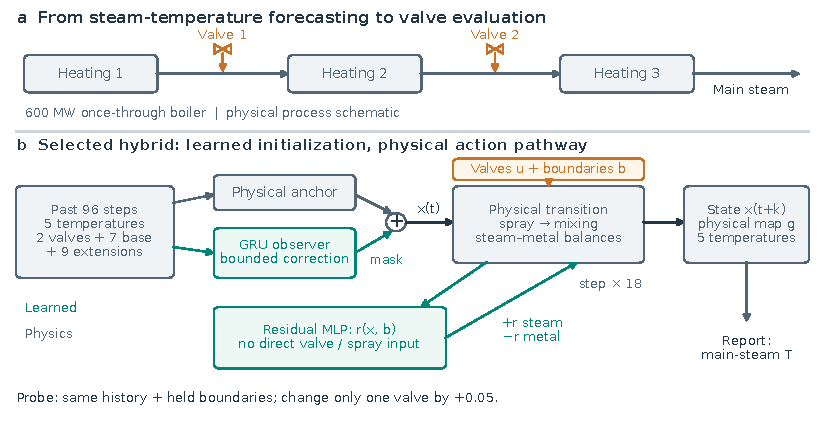
\includegraphics[width=\linewidth]{figures/fig1_architecture_en.pdf}
\caption{\textbf{The physical transition carries the action; neural modules complete the model.}
The selected hybrid uses a past-only GRU and a bounded power closure (green).
Valve-driven spray, transport, mixing and steam--metal balances define the
grey-box rollout. The closure has no direct valve or measured spray-flow input,
but depends on action-dependent states. Forecast and probe share weights and
initialization. The diagram shows the mean path; rewetting is ablated in this hybrid.}
\label{fig:model}
\end{figure}

\paragraph{State and inputs.}
The history $\mathcal H_t$ contains 96 samples at 10\,s intervals: five temperatures,
two valves, seven base boundaries and nine history-only extensions (23 variables).
The 11-dimensional physical state contains three steam enthalpies, three metal
temperatures, fuel lag, two liquid inventories and two spray-transport states.
Valve positions determine spray flows, which affect downstream temperatures
through transport and enthalpy mixing (Figure~\ref{fig:model}). A thermodynamic
observation map produces five temperatures; our reported target is main steam.

\paragraph{Anchored initialization and heat closure.}
Five observed temperatures cannot specify every physical state. Their observation
relations define a steady anchor $x_{\rm anc}$; a GRU supplies bounded corrections:
\begin{align}
x_t &= x_{\rm anc}(\mathcal H_t)+M[0.1s_x\odot\tanh d_\phi(\mathcal H_t)],\label{eq:init}\\
r_k &= R\tanh f_\theta(x_k,b_{k+1}^{\rm allow}),\quad
x_{k+1}=\Phi_\psi(x_k,u_{k+1},b_{k+1};r_k),\label{eq:trans}\\
\hat y_{k+1}&=g_\psi(x_{k+1},b_{k+1}).\label{eq:obs}
\end{align}
Here $s_x$ denotes fixed state scales; $M$ selects metal temperatures and fuel lag,
leaving fast states anchored. The closure adds $r_j$ to steam and $-r_j$ to metal
power in each segment, with $R=30{,}000$\,kW. These are internal corrections, not
an additive temperature-prediction head. Trainable physical parameters and
2\,s semi-implicit substeps complete the transition. Rewetting gains are pinned
near zero in both hybrid candidates; the grey-box reference retains rewetting.

\paragraph{Shared transition, bounded claim.}
At fixed history and boundaries, the diagnostic is
$\widehat{\Delta T}_{1:H}=\hat T(\mathcal H_t,u^+,b)-\hat T(\mathcal H_t,u^0,b)$.
Identical actions must yield identical outputs. Excluding direct valve and
spray-flow inputs from $f_\theta$ prevents that direct shortcut, not state-mediated
action dependence. Opposite power injections likewise do not guarantee correct
response magnitudes. A token candidate replaces only the GRU observer with
variable--time patches and state-query cross-attention; the physical rollout
and closure remain unchanged (Appendix~\ref{app:implementation}).

\clearpage
\section{A focused, frozen comparison}\label{sec:protocol}

\paragraph{Data and common evaluation.}
One process side supplies 707,709 samples (about 82 days), split chronologically
75/15/10. We use internal validation only; the final test segment remains locked.
Protocol revision 0.2 was frozen before this round of training, but earlier
validation experiments informed its design. All four arms and seeds 0--2 use the
same sampled 20,000-window training bank, 256 prediction windows and 64 response
histories. The two evaluation sets each span 13 UTC days. Eligibility is fixed
by valid base channels, finite in-range historical extensions and exact 10\,s
continuity. No results-based window filtering is applied.

Prediction supplies the recorded future valves and seven base boundaries over
18 steps. This is an \emph{oracle-conditioned} comparison, not prospective
forecasting with unknown future boundaries. The nine extensions, including
water--coal ratio and load, are strictly history-only. Their normalization uses
training rows only. The prediction metric is cumulative main-steam MAE,
\begin{equation}
E_H=\frac{1}{3}\sum_{s=0}^2\frac{1}{|\mathcal D|}\sum_{d\in\mathcal D}
\frac{1}{n_d H}\sum_{i\in d}\sum_{h=1}^{H}|\hat T^{(s)}_{i,h}-T_{i,h}|.
\label{eq:metric}
\end{equation}
Thus days, then seeds, receive equal weight; H18 averages 10--180\,s, rather than
measuring only the endpoint. Table~\ref{tab:prediction} gives seed variability.

\begin{table}[!ht]
\centering\small
\begin{tabular}{lccc}
\toprule
Method & H1 & H6 & H18\\
\midrule
Persistence (shared reference) & $0.085$ & $0.268$ & $0.639$\\
Black box (variable tokens) & $0.100\pm0.013$ & $0.191\pm0.011$ & $0.371\pm0.007$\\
Grey box (steady, no closure) & $0.224\pm0.003$ & $0.529\pm0.007$ & $0.969\pm0.008$\\
Hybrid GRU (selected) & $0.093\pm0.007$ & $0.224\pm0.014$ & $0.443\pm0.022$\\
Hybrid token (candidate) & $0.111\pm0.004$ & $0.306\pm0.019$ & $0.654\pm0.048$\\
\bottomrule
\end{tabular}
\caption{\textbf{Main-steam prediction under the v0.2 information contract.}
Cumulative MAE in \degc{}, equal-day mean then three-seed mean $\pm$ sample
standard deviation; persistence is shared and deterministic. H1/H6/H18 correspond to 10/60/180\,s. These are
validation-selected, fixed-budget results, not locked-test estimates.}
\label{tab:prediction}
\end{table}

\paragraph{Methods, not a fully matched architecture ablation.}
The black box is an iTransformer-inspired variable-token forecaster~\cite{liu2024itransformer},
adapted to accept future covariates; it is not a reproduction of the published
steam-temperature model. It and both observers receive the same 23 historical
variables. The grey box has no learned observer or closure and consumes only
the physical subset. The black box also consumes future measured total spray,
which the action-driven physical transition ignores. Structured models train
with five-temperature Gaussian NLL (24,000-update cap, batch 32); the black box
uses main-steam MSE (3,000 updates, batch 128). All 12 runs reach their caps;
reported checkpoints minimize validation H18 MAE. Information, loss, budget
and rewetting differences preclude attributing cross-family differences to
one architectural component.

\paragraph{Selection and response protocol.}
The token observer advances only if it improves H18 MAE in at least two of
three paired seeds, has no higher seed-mean MAE and satisfies implementation
gates. Valve responses are not selectors. For each probe, both valves and
boundaries are held at their last historical values; one valve is increased by
0.05 of full opening, capped at 1.0. All realized doses are 0.05 within floating-point
precision. Responses are equally averaged by day, then seed. All 64 histories
pass the registered history-range-plus-0.05 support check for both valves;
this marginal range check does not establish conditional excitation or joint
counterfactual support. No field intervention truth is available.

\clearpage
\section{Results: prediction cost and model responsiveness}\label{sec:results}

\begin{figure}[!ht]
\centering
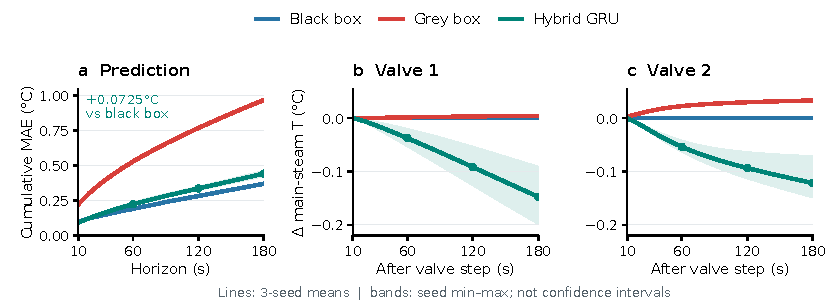
\includegraphics[width=\linewidth]{figures/fig2_prediction_response_en.pdf}
\caption{\textbf{The accuracy ranking does not describe the valve-response curves.}
(a) Cumulative main-steam MAE on 256 common prediction windows.
(b,c) Step-minus-base main-steam response on 64 common histories, fixed boundaries,
one valve increased by 0.05. Lines average days then three seeds; bands show seed
min--max, not confidence intervals. Both response panels share the same scale.
All registered windows are retained. The responses are model outputs, not observed plant gains.}
\label{fig:evidence}
\end{figure}

\paragraph{A measurable forecast cost, not an accuracy win.}
The GRU hybrid's H18 MAE is 0.443\degc{}, versus 0.371\degc{} for the black box:
+0.0725\degc{} (19.6\%). It is 54.3\% lower than the grey-box reference's
0.969\degc{}. The ordering is horizon-dependent: GRU has slightly lower mean
H1 error, but higher H6 and H18 error (Table~\ref{tab:prediction}). Paired
day-block intervals put the hybrid--black-box H18 difference above zero in
two seeds; the third includes zero. These intervals are descriptive after
validation selection, not selection-adjusted tests (Appendix~\ref{app:stats}).

\paragraph{The best forecaster is nearly insensitive in this diagnostic.}
At 180\,s the black box's seed-mean responses are approximately
$+0.00010$ and $+0.00073$\degc{} for valves 1 and 2. The GRU hybrid instead
produces $-0.147$ and $-0.122$\degc{}, with delayed cooling curves
(Figure~\ref{fig:evidence}). Its H18 responses are negative in all seeds for
both valves, and all six endpoint day-block intervals exclude zero. The grey
box produces $+0.00448$ and $+0.03305$\degc{}: a physical state representation
alone does not ensure the expected cooling direction in these fitted models.
Because grey-box and hybrid rewetting configurations differ, this is not an
isolated proof that the neural components repair the sign. Nor do near-zero
black-box responses prove an error relative to an unmeasured plant gain.

\paragraph{A more elaborate observer does not improve the compromise.}
Token H18 MAE is 0.654\degc{}, 47.7\% above GRU; it is worse in every seed and
fails the predeclared advancement rule; its mean also exceeds persistence (0.639\degc{}). Its negative valve responses do not
override that outcome. We therefore retain GRU. This is a bounded negative
result for this patch/query observer and budget, not evidence against
Transformers generally (Appendix~\ref{app:ablation}).

\section{Discussion and conclusion}
Our model combines learned thermal-state and heat corrections with an explicit,
shared physical action pathway. The present evidence locates a candidate
compromise---0.0725\degc{} higher prediction error than the black box alongside
non-negligible cooling responses---not a calibrated optimum or a Pareto frontier.
Oracle inputs and reused validation limit generalization claims; differences
between model families limit causal architectural attribution. A matched
no-rewetting grey-box control is now separately registered but pending;
independent test and plant-response calibration remain outstanding.
For temporal world models intended to evaluate actions, forecast error and
action response should be reported together; neither the forecasting leaderboard
nor physical structure alone establishes decision readiness.

\label{maintext:end}
\clearpage
\bibliographystyle{plainnat}
\bibliography{references}
\clearpage
\appendix
\section{Implementation and information access}\label{app:implementation}

\paragraph{Physical model.}
The packed state is $(h_1,h_2,h_3,T_{m1},T_{m2},T_{m3},r_b,m_{\ell1},m_{\ell2},
d_{sw1},d_{sw2})$. Temperature--enthalpy relations use a tabulated IAPWS
property grid. The observation map reads physical states and supplied boundaries;
there is no separate neural mean-temperature head. The steady anchor uses
physical observation inversion. The hybrid corrects only metal temperatures
and fuel lag; all three steam enthalpies and both liquid/transport pairs retain
their anchored initial values. Mean corrections are bounded by 0.1 times fixed
state scales. Zero-initialized observer heads return the anchor exactly.
Five 2\,s substeps form one 10\,s sample step. The closure is recomputed at the
current state of each substep; Equation~\ref{eq:trans} abbreviates this composition.

\paragraph{Closure restrictions.}
A two-hidden-layer tanh MLP returns three bounded power corrections, one per
segment. The conservative mode applies equal and opposite steam/metal injections.
Inputs are normalized physical state and six allowed base boundaries, excluding
measured total spray. There are no additional latent dimensions or stochastic
closure inputs in this round. Input exclusion is a direct-interface property:
states already depend on earlier actions. With $S_k=\partial x_k/\partial\epsilon$
under an action perturbation, the local chain rule includes
\[
S_{k+1}=(\Phi_x+\Phi_r r_x)S_k+\Phi_u\,
\frac{\partial u_{k+1}}{\partial\epsilon},\qquad S_t=0.
\]
Thus the learned closure can still modify sensitivities through the state.
The opposite injections constrain where residual heat enters, but do not prove
parameter identifiability, numerical stability in every regime, or true gain recovery.

\paragraph{Observer candidate.}
Both hybrid observers have hidden width 128. The candidate patches each of 23
historical variables with patch length 16 and stride 8 (11 patches per variable,
253 tokens). Linear patch embeddings plus variable and patch embeddings enter
one four-head Transformer encoder; 11 learned state queries cross-attend to
its output. Per-state correction heads receive the query features and pressure
features. The GRU and candidate share the correction bound, state mask,
physical transition, closure, historical extensions and seed-specific training
draws. The token candidate uses no future-history tokens. This is an observer
replacement, not an end-to-end replacement of physical dynamics by attention.

\paragraph{Black box.}
Inspired by variable-token forecasting~\cite{liu2024itransformer}, a linear
96-to-64 projection embeds each of 23 historical channels. A separate 18-to-64
projection embeds each of nine supplied future channels (two valves, seven
base boundaries). Two four-head Transformer layers process the 32 tokens;
a flattened linear head predicts 18 main-steam deviations from the historical
main-steam mean. Dropout is 0.1 and feedforward width is 128. This local adapted
baseline should not be confused with a reproduction of the original benchmark
architecture or the physics-guided steam-temperature predictor~\cite{zhang2026sst}.

\begin{table}[!ht]
\centering\small
\begin{tabular}{lrrrr}
\toprule
Property & Black box & Grey box & Hybrid GRU & Hybrid token\\
\midrule
Historical extensions consumed & 9 & 0 & 9 & 9\\
Learned observer & --- & --- & GRU & Patch/query\\
Neural power closure & --- & None & Conservative & Conservative\\
Rewetting & --- & Enabled & Ablated & Ablated\\
Parameters receiving gradients & 111,250 & 99 & 65,808 & 278,248\\
Update cap & 3,000 & 24,000 & 24,000 & 24,000\\
Batch size & 128 & 32 & 32 & 32\\
Validation frequency (updates) & 500 & 200 & 200 & 200\\
Patience (evaluations) & 3 & 20 & 20 & 20\\
\bottomrule
\end{tabular}
\caption{Executed configuration, not a capacity- or compute-matched benchmark.
Active counts exclude instantiated but bypassed networks. In structured models,
observation uncertainty parameters can receive gradients through NLL.}
\end{table}

\section{Data contract, estimator and provenance}\label{app:stats}

The seven base channels are steam flow, coal command, separator pressure,
separator temperature, feedwater temperature, outlet pressure and total spray
flow. The nine extensions are corrected fuel, active mill count, weighted mill
gas temperature, flue oxygen, total secondary air, reheater gas inlet temperatures
A/B, water--coal ratio and unit load. They inform history only: no recorded
future extension is passed into any arm. Water--coal ratio is a covariate, not
an additional physical power correction. Its isolated benefit is not identified
without a feature ablation.

The physical model uses fixed engineering scales for base channels. Extensions
use shared training-only means and standard deviations. The black box uses
training-only statistics for all historical channels and the historical target
mean for its output offset; its supplied future base covariates are not normalized
by that historical transform. Future total spray is visible to the black box but
ignored by action-driven physics. Holding it fixed during a valve change defines
the diagnostic input, not a self-consistent plant counterfactual. These details
are reasons to interpret the experiment as a comparison of complete methods.

Training draws use a fixed 20,000-window bank sampled with replacement. Validation
and response manifests use seeds 30,000 and 60,000; the training-bank seed is
15,000. Each training seed controls initialization and subsequent minibatch
draws. All models share identical validation targets, timestamps and starts;
all probes share starts, valve doses and support masks. The prediction set has
256 windows and the probe set 64 histories, each covering 13 UTC days. Overlapping
windows are possible; windows are not treated as independent experimental units.

For each seed, paired H18 error differences are averaged within UTC day.
The 13 daily values are resampled with replacement 1,000 times, RNG seed 11,000;
the 2.5th/97.5th percentiles form the reported interval. The same procedure
applies pointwise to response curves. These intervals quantify day variation
conditional on the selected checkpoints. They are not adjusted for checkpoint
selection, previous validation reuse, multiple comparisons, or cross-day serial
dependence. We do not treat three seeds as independent plants. Figure bands
instead show the min--max range of three seed-level daily means.

\begin{table}[!ht]
\centering\small
\begin{tabular}{lccc}
\toprule
H18 candidate minus reference (\degc{}) & Seed 0 & Seed 1 & Seed 2\\
\midrule
GRU $-$ black box & $0.068$ & $0.046$ & $0.104$\\
95\% day-block interval & $[0.027,0.108]$ & $[-0.002,0.093]$ & $[0.067,0.137]$\\
GRU $-$ grey box & $-0.537$ & $-0.541$ & $-0.500$\\
95\% day-block interval & $[-0.784,-0.318]$ & $[-0.756,-0.341]$ & $[-0.725,-0.299]$\\
Token $-$ GRU & $0.267$ & $0.212$ & $0.154$\\
95\% day-block interval & $[0.210,0.329]$ & $[0.155,0.269]$ & $[0.119,0.193]$\\
\bottomrule
\end{tabular}
\caption{Paired descriptive intervals, independently recalculated from saved arrays.
No selection-adjusted or confirmatory significance claim is made.}
\end{table}

The registered action support check expands each valve's historical marginal
minimum/maximum by 0.05 and checks both base and perturbed sequences. All
64 histories pass for each valve; no history was discarded. This permissive
axis-aligned check does not test joint state--action support, conditional
excitation or the realism of holding all supplied boundaries fixed.
There is therefore no distinct supported-only curve in this round: it would be
identical to the primary curve.

\paragraph{Artifact audit.}
The returned bundle contains 12 checkpoints, training ledgers and 24 raw
prediction/response arrays. A local read-only audit verifies artifact hashes,
checkpoint-to-input-identity binding and common index pairing. An independent
saved-array reduction checks all source fingerprints, recalculates every
prediction curve, response curve and paired interval, and recovers the same
selected hybrid. Input, mapping and thermodynamic-grid fingerprints are retained
in the internal audit record. The execution-side return reports 24 inference
array replays; that statement was not independently rerun from the plant record
in this manuscript-preparation pass. No training or test evaluation was performed
to prepare this draft. The audit verifies the returned evidence, not the
truth of an unmeasured plant intervention response.

\section{Observer selection and per-seed diagnostics}\label{app:ablation}

\begin{figure}[!ht]
\centering
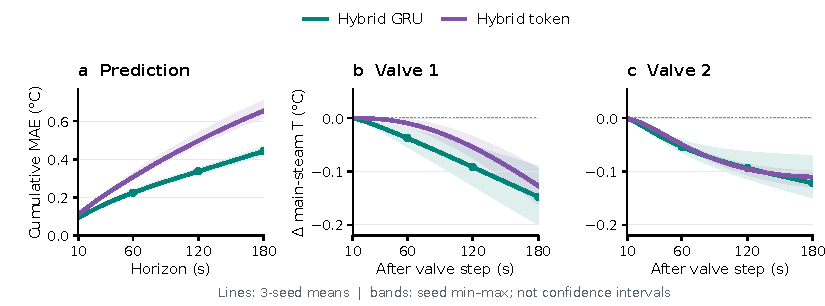
\includegraphics[width=\linewidth]{figures/figS1_observer_ablation_en.pdf}
\caption{\textbf{The token observer does not advance.} Identical physical configuration,
history contract and evaluation manifests; the observer architecture changes.
Token prediction error exceeds GRU at H18 in all seeds, while both have negative
mean endpoint responses. Responses are not model-selection criteria.
Lines and bands use the same definitions as Figure~\ref{fig:evidence}.}
\end{figure}

\begin{table}[!ht]
\centering\small
\begin{tabular}{lrrrr}
\toprule
Method / seed & H18 MAE & Valve 1 H18 & Valve 2 H18 & Best update\\
\midrule
Black box / 0 & 0.3735 & $+0.000013$ & $+0.001335$ & 3,000 \\
Black box / 1 & 0.3756 & $-0.000025$ & $+0.000678$ & 2,500 \\
Black box / 2 & 0.3628 & $+0.000305$ & $+0.000183$ & 3,000 \\
Grey box / 0 & 0.9787 & $+0.004601$ & $+0.032581$ & 23,800 \\
Grey box / 1 & 0.9623 & $+0.004401$ & $+0.033384$ & 24,000 \\
Grey box / 2 & 0.9668 & $+0.004435$ & $+0.033175$ & 24,000 \\
Hybrid GRU / 0 & 0.4414 & $-0.198801$ & $-0.145255$ & 21,000 \\
Hybrid GRU / 1 & 0.4216 & $-0.090115$ & $-0.070247$ & 23,600 \\
Hybrid GRU / 2 & 0.4664 & $-0.152901$ & $-0.149205$ & 21,000 \\
Hybrid token / 0 & 0.7086 & $-0.161024$ & $-0.099171$ & 23,800 \\
Hybrid token / 1 & 0.6340 & $-0.094119$ & $-0.128567$ & 23,600 \\
Hybrid token / 2 & 0.6203 & $-0.125057$ & $-0.102259$ & 22,000 \\
\bottomrule
\end{tabular}

\caption{Seed-level daily means in \degc{}; prediction is cumulative H18 MAE,
response is the H18 endpoint difference, not the last-ten-step metric used in
earlier development. All runs terminate at their caps.}
\label{tab:seeds}
\end{table}

For GRU, the valve-1 endpoint intervals for seeds 0/1/2 are respectively
$[-0.229,-0.167]$, $[-0.105,-0.075]$, $[-0.176,-0.128]$\degc{};
valve-2 intervals are $[-0.168,-0.119]$, $[-0.083,-0.057]$, and
$[-0.172,-0.123]$\degc{}. They support a negative model response under this
probe. Small black-box differences are close to the numerical granularity of
large absolute-temperature predictions; we neither equate them with exactly
zero nor interpret a ratio to them as a physical amplification factor.

\section{Design history and remaining evidence boundaries}

Earlier development investigated initial-state flexibility, residual placement,
boundary prediction and rewetting diagnostics. Those comparisons used different
output aggregations or information contracts; their MAEs are not pooled with
the present main-steam-only metric. They motivated the anchored hybrid and
no-rewetting candidate, but are not confirmatory replications of this new
comparison. In particular, a prior five-temperature average and a current
main-steam-only average are not interchangeable, and earlier H60 probes do not
extend the present registered 180\,s evidence.

The remaining questions require different evidence. A one-time locked-test
evaluation can address temporal generalization after selection, but not true
intervention gains. A matched grey-box no-rewetting comparison would isolate
the effect of adding the observer/closure more cleanly than the present
cross-family contrast. Independently calibrated intervention or suitably
identified natural-experiment responses would address plant-response magnitude.
History-only prediction with forecast rather than recorded future boundaries
would address prospective use. After examining the present results, the
no-rewetting grey-box control has been separately registered with three seeds
and the original budget; it remains pending. Other checks remain proposals,
not completed results or silent changes to the existing protocol.

\paragraph{Data availability and anonymization.}
The data describe an operating industrial process. Public release authorization
for raw plant records has not been established; this draft makes no promise of
open raw data. Numerical figure sources, experiment configuration and audit
records exist locally. An anonymous sharing package and its permissions must
be confirmed before submission; private repository links and site identity are
not included here.

\paragraph{Use of language-model assistance.}
Language-model tools assisted manuscript organization, translation, figure-script
development and consistency checks against saved results. They were not used as
a substitute for plant-response measurements. Human authors remain responsible
for the final scientific claims, numerical verification and submission.

\end{document}
